% !TeX root = 00General.tex
\thispagestyle{standard}
\pagestyle{standard}
\chapter{Ausgangslage}

Ziel dieser Laboreinheit ist es ein \ac{MPLS}-VPN zu konfigurieren. Dabei soll das ein VPN zwischen den Gruppenteilnehmer aufgebaut werden. Um dies über ein Providernetz zu ermöglichen wird \ac{BGP} eingesetzt. 

\chapter{Topologie}

Die Topologie (nachgebaut in Packet Tracer) ist in Abbildung \ref{img:topo} zu sehen.

\begin{figure}[H]
	\centering
	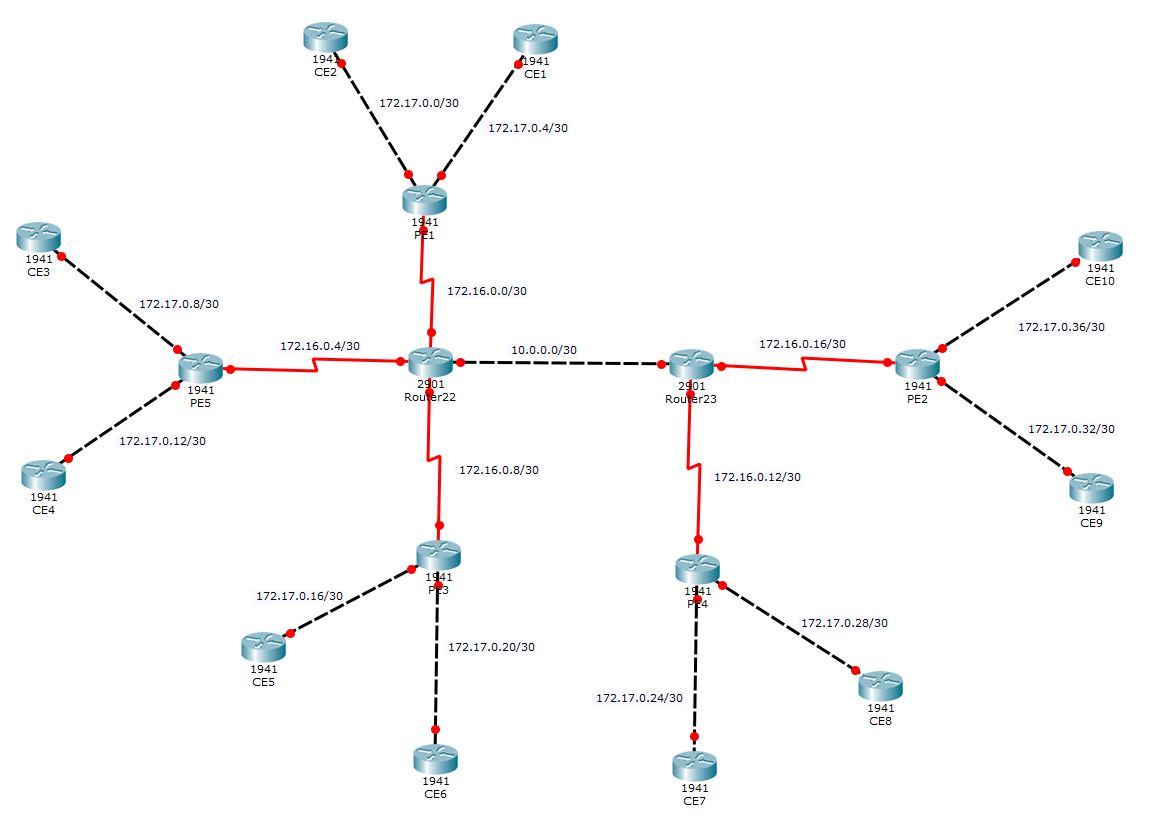
\includegraphics[width=0.9\textwidth]{img/Topologie.JPG}
	\caption{Topologie}
	\label{img:topo}
\end{figure}

Jeder Gruppe wurde ein Provider-Edge-Router (PEx) samt zwei Kunden-Routern (CEx) zugewiesen. Der Traffic der Kundenrouter sollte voneinander abgeschirmt sein, sodass auch IP-Adressbereiche mehrfach vergeben werden können, ohne dass es zu Adresskonflikten kommt.


Die Router P1 und P2 wurden keiner Gruppe explizit zugewiesen, ihre Konfiguration wurde gemeinsam erledigt.

\chapter{OSPF und BGP}

Zwischen den Provider-Edge und dem P-Router wurde OSPF als Routingprotokoll konfiguriert, sowie \ac{MPLS} auf allen Links aktiviert.

\lstset{escapeinside={\%*}{*)},numbers=left}%oder numbers=left
\begin{lstlisting}[caption={PE5, MPLS und OSPF-Konfiguration},label={lst:mon},language={}]
interface Serial0/0/0
  ..
  mpls ip
  ..
  
router ospf 1
 network 5.5.5.5 0.0.0.0 area 0
 network 172.16.0.4 0.0.0.3 area 0
!
\end{lstlisting}

Alle Netze wurden in den Routing-Prozess eingetragen. Wichtig hierbei war eine Loopback-Adresse (5.5.5.5). Diese wird in einem nächsten Schritt als Quelladresse für Routing-Updates mittels \ac{BGP} verwendet.


\section{VRF}

Mittels \ac{VRF} werden die Netze der Kunden voneinander getrennt, hierfür wird ein "virtueller" Router auf PE5 eingerichtet. Das Route-Target ist dabei gleich für alle Teilnehmer des VPNs. "65000" entspricht in dem Fall einem \ac{AS}.

\lstset{escapeinside={\%*}{*)},numbers=left}%oder numbers=left
\begin{lstlisting}[caption={VRF CE3},label={lst:mon},language={}]
ip vrf ce3
 rd 65000:3
 route-target export 65000:3
 route-target import 65000:3
!
\end{lstlisting}

Pro Kunde existiert ein eigener Routing-Prozess, hier ebenfalls mittels \ac{OSPF} realisiert.

\lstset{escapeinside={\%*}{*)},numbers=left}%oder numbers=left
\begin{lstlisting}[caption={OSPF für CE3},label={lst:mon},language={}]
router ospf 2 vrf ce3
 router-id 5.5.5.3
 redistribute bgp 65000 subnets
!
\end{lstlisting}


\chapter{Monitoring}

\section{Switch}

Der \ac{BGP} und \ac{MPLS}-Traffic sollte mitgeschnitten werden.
Dazu wurde zwischen Router P1 und P2 ein Switch dazwischengesschaltet. Auf diesem Switch wurde anschließend ein Monitoring-Port (bei Cisco auch Span-Port genannt) eingerichtet.

Anschließend konnte ein angeschlossener PC den Traffic mittels Wireshark mitschneiden.

\lstset{escapeinside={\%*}{*)},numbers=left}%oder numbers=left
\begin{lstlisting}[caption={Monitoring-Ports},label={lst:mon},language={}]
monitor session 1 source interface Fa0/1
monitor session 1 destination interface Fa0/3 , Fa0/10
\end{lstlisting}

In Listing \ref{lst:mon} sieht man die Konfiguration des Monitor-Ports. Traffic der von und an Port Fa0/1 geschickt wird, wird auch an den Ports Fa0/3 und Fa0/10 ausgegeben.

\section{Wireshark}

Ein Beispiel für \ac{MPLS}-Traffic ist in Abbildung \ref{img:icmp} zu sehen. Erkennbar sind die MPLS-Labels zwischen Layer 2 und 3. Gesendet wird ein Ping.

\begin{figure}[H]
	\centering
	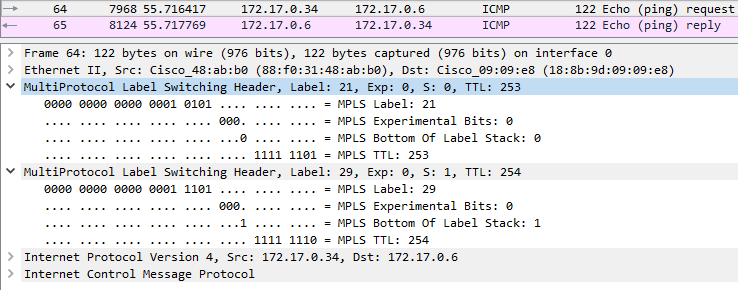
\includegraphics[width=0.9\textwidth]{img/icmp_wireshark.png}
	\caption{ICMP über MPLS}
	\label{img:icmp}
\end{figure}

\begin{figure}[H]
	\centering
	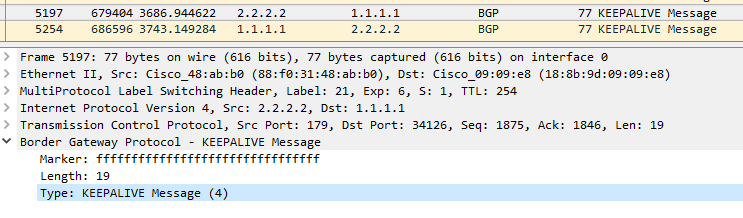
\includegraphics[width=0.9\textwidth]{img/bgp_wireshark.png}
	\caption{BGP-Keepalive}
	\label{img:bgp}
\end{figure}

In Abbildung \ref{img:bgp} sind \ac{BGP}-Keepalive-Nachrichten zu sehen die periodisch ausgetauscht werden, ebenfalls über den \ac{MPLS}-Tunnel.

\section{Traceroutes}

Mittels \texttt{traceroute} kann die Route zu einem Zielhost festgestellt werden. Führt man diesen Befehl am Router aus (Abbildung \ref{img:trace_router}), so sieht man ebenfalls den \ac{MPLS}-Tunnel, auf einem Endgerät (Abbildung \ref{img:trace_win}) ist diese Information nicht sichtbar, da die MPLS-Label am Zielgerät nicht mehr im Frame vorhanden sind.

\begin{figure}[H]
	\centering
	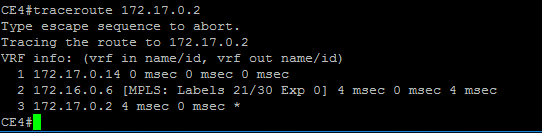
\includegraphics[width=1.0\textwidth]{data/traceroute_router.PNG}
	\caption{Traceroute-Router}
	\label{img:trace_router}
\end{figure}

\begin{figure}[H]
	\centering
	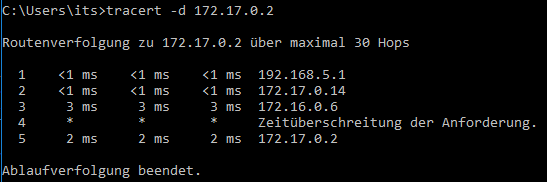
\includegraphics[width=1.0\textwidth]{data/traceroute_windows2.PNG}
	\caption{Traceroute-Windows}
	\label{img:trace_win}
\end{figure}